\subsection{The \texorpdfstring{$\alpha$}{alpha}-Rank Method}

    Evolutionary dynamics studies how agents' interactions in multi-agent settings evolve over time. While single-agent systems have acquired a strong foundation over the years \cite{10.5555/2831071.2831085}, multi-agent systems are more challenging to analyze.\tinydouble

    \noindent
    Current literature indicates a growing interest in studying the evolutionary dynamics of multi-agent systems. Although one might view evolutionary algorithms as mere tools for agents' hyper-parameter tuning \cite{Sinha_2023}\cite{ganapathy2020studygeneticalgorithmshyperparameter}, their contributions extend far beyond that. In the context of games, evolutionary algorithms are widely used to explore game-theoretic solution concepts. This area of study is also known as \emph{Evolutionary Game Theory} (EGT). An example of research in this field is the work reported in \cite{paul2022multiagentpathfinding}, which introduced an evolutionary algorithm for multi-agent path-finding in stochastic environments. This approach showed significant improvements in minimizing path length and computational efficiency, outperforming state-of-the-art reinforcement learning algorithms. In another work \cite{David_2014}, a novel approach was introduced for evolving the key components --mainly the evaluation function and search mechanism-- of a chess program from randomly initialized values using genetic algorithms. By learning from databases of grand-master games, the program managed to outperform a world chess champion computer.\tinydouble
    
    \noindent
    Building on work done in EGT, the evolutionary methodology \emph{$\alpha$-Rank} \cite{omidshafiei2019alpharank} introduces a novel game-theoretic approach to provide insights into the long-term dynamics of agents' interactions. At its core, \emph{$\alpha$-Rank} is designed to evaluate and rank strategy profiles in large-scale multi-agent interactions, using a new dynamic solution concept called \emph{Markov-Conley chains} (MCCs). It achieves this by calculating a stationary distribution from the transition probabilities between strategy profiles, reflecting how much time agents spend using each profile. This stationary distribution is then used to rank the strategy profiles, with the ranking intensity $\alpha$ adjusting the sensitivity of the rankings to the stability of the strategies over time.
    %

    \subsubsection{Markov-Conley Chains}

        \emph{Markov-Conley chains} (MCCs) are a dynamic solution concept that extends the traditional idea of Nash equilibrium by considering the evolution of strategies over time, rather than focusing solely on fixed points. MCCs model the long-term behavior of agents’ interactions within a dynamical system to identify stable components where agents reach equilibria. They provide a more dynamic perspective on stability by shifting the focus from static points, where no player benefits from unilaterally changing their strategy, to trajectories that define how equilibrium is reached over time.\tinydouble

        \noindent
        To better understand the structure of MCCs, we can view the dynamics of agent interactions as flows within a topological space, where each strategy is represented as a point in this space. These flows describe how the system evolves over time, with the state of the system at any given moment depending solely on the current strategy, as defined by the Markov property:
        %
        \begin{equation}
            P(str_{t+1} = str_j \mid str_t = str_i) = P(str_{t+1} = str_j \mid str_t = str_i, str_{t-1}, \dots)
            \label{eq:markov_property}
        \end{equation}
        %
        where $P(str_{t+1} = str_j \mid str_t = str_i)$ represents the probability of transitioning from strategy $str_i$ to $str_j$ at time $t+1$, independent of past strategies. These dynamics can be expressed mathematically using a flow $\phi_t$ defined on a topological space $X$:
        %
        \begin{equation}
            \phi_t: X \rightarrow X
            \label{eq:flow_phi}
        \end{equation}
        %

        \noindent
        For each time step $t \in \mathbb{R}$, the flow maps a point $x \in X$ to another point in the space, $\phi_t(x)$. This mapping represents the evolution of the agent’s strategy over time, with $x$ being the current strategy and $\phi_t(x)$ the updated one at time $t$.\tinydouble
        
        \noindent
        This concept is further supported by \emph{Conley's Fundamental Theorem of Dynamical Systems}, which divides the state space into recurrent sets, representing stable behaviors, and transient points that eventually lead to recurrent sets \cite{conley1978isolated}\cite{Norton1995}. These recurrent sets, including fixed points, periodic orbits, and limit cycles, correspond to different forms of equilibrium. In the context of multi-agent games, the long-term dynamics of agent interactions can be modeled similarly, where each point in the space corresponds to a joint strategy (strategy profile). Specifically, these dynamics can be visualized through a graph, known as the \emph{response graph}, where each node represents a strategy profile and edges represent transitions between them. The main structures in this graph are the \emph{strongly connected components} (SCCs), which correspond to the recurrent sets in the topological space. Once players enter these components, they tend to remain, indicating an equilibrium \cite{omidshafiei2019alpharank}.
        
        \paragraph{Chain Recurrent Set}

            The \emph{chain recurrent set} $\mathcal{R}_\phi$ of the flow $\phi_t$ is the set of all points $x \in X$ that are chain recurrent under the flow $\phi_t$. A point $x$ is chain recurrent if there exists an $(\epsilon, T)$-chain from $x$ to itself, meaning there exists a sequence of points $(x_0, x_1, \dots, x_n)$ connecting back to $x$, with each step being arbitrarily close to the previous one.

            \begin{definition}[Chain recurrent point]
                An $(\epsilon, T)$-chain from $x$ to itself, with respect to the flow $\phi_t$ and distance function $d$, is a sequence $(x_0, x_1, \dots, x_n)$ such that:
                %
                \begin{equation}
                    d(\phi_{t_i}(x_i), x_{i+1}) < \epsilon \quad \text{for each} \quad i = 0, 1, \dots, n-1, \quad t_i \geq T
                    \nonumber
                \end{equation}
                %
                where $\epsilon > 0$ represents the allowed perturbation at each step, and $T > 0$ is the minimum time-step between transitions. If such a chain exists from $x$ back to itself, the point $x$ is chain recurrent.
            \end{definition}

        \paragraph{Transient Points}

            A point $x \in X$ is called \emph{transient} if it is not chain recurrent. This means that there does not exist an $(\epsilon, T)$-chain from $x$ to itself, and trajectories starting from a transient point eventually leave every neighborhood of $x$ without returning. Transient points do not exhibit any form of cyclic behavior; they eventually \emph{escape} from their initial region.
        
            \begin{definition}[Transient point]
                A point $x \in X$ is transient if $x \notin \mathcal{R}_\phi$.
            \end{definition}

        \noindent
        To visualize the flow representation of strategy evolution in agent interactions, consider the \emph{Coordination Game} in Table~\ref{tab:coordination_game}. This is a cooperative game where both players benefit from coordinating on the same strategy, $A$ or $B$, rather than playing different strategies. Figure~\ref{fig:coordination_game} illustrates the replicator dynamics of the agents' strategies in a graph, as designed by the authors in \cite{omidshafiei2019alpharank}.
        %
        \begin{figure}[H]
            \centering
            \begin{minipage}{0.45\textwidth}
                \centering
                \vspace{1.4cm}
                \begin{tabular}{c|c|c}
                    & A & B \\ \hline
                    A & 1,1 & -1,-1 \\
                    B & -1,-1 & 1,1 \\
                \end{tabular}
                \vspace{1.4cm}
                \subcaption{Payoff matrix.}
                \label{tab:coordination_game}
            \end{minipage}
            \hspace{0.1em}
            \begin{minipage}{0.45\textwidth}
                \centering
                \resizebox{0.6\textwidth}{!}{
                    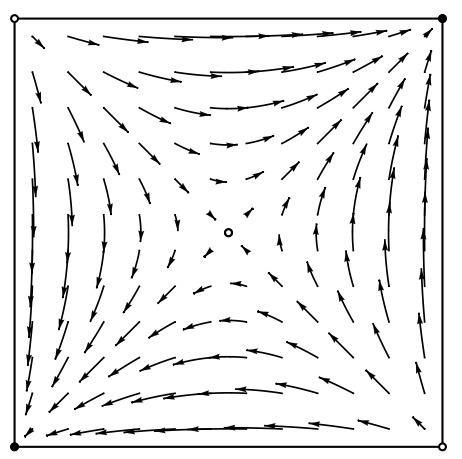
\includegraphics{images/coordination-game.png}
                }
                \subcaption{Response Graph.}
                \label{fig:coordination_game_dynamics}
            \end{minipage}
            \caption{Payoff matrix (a) and Replicator dynamics (b) in the Coordination Game.}
            \label{fig:coordination_game}
        \end{figure}
        %

        \noindent
        Each point in the graph corresponds to a mixed strategy profile for the two players, while the arrows represent the flow of strategy profiles over time. The recurrent points in the graph (bottom-left and top-right corners) correspond to the two stable profiles: $(A,A)$ and $(B,B)$. These two recurrent points represent the attractors of the system, where the flows converge. On the other hand, $(A,B)$ and $(B,A)$ (top-left and bottom-right corners) are the transient points of the graph. The flow field directs trajectories away from these points, indicating their instability. Finally, the middle point in the graph represents a mixed strategy profile where both players assign equal probability to strategies $A$ and $B$ (i.e., 50\% for each in the probability distribution). Trajectories near this point diverge, moving towards one of the two recurrent points. This behavior represents the mixed-strategy Nash equilibrium of the \emph{Coordination Game}.\tinydouble

        \noindent
        To distinguish between recurrent sets and transient points in a dynamical system, the creators of \emph{$\alpha$-Rank} use a complete \emph{Lyapunov function} \cite{lyapunov1950}. This function, $\gamma: X \to \mathbb{R}$, assigns values to points in the space such that:
        %
        \begin{itemize}
            \item For transient points, the value of $\gamma(\phi_t(x))$ strictly decreases over time as the system evolves along the flow $\phi_t$. This reflects how transient points are driven towards the recurrent part of the space.
            \item For points within the recurrent set $\mathcal{R}_\phi$, $\gamma(\phi_t(x))$ remains constant. This signifies that all points within the same chain component share equivalent dynamic properties.
        \end{itemize}
        %

        \noindent
        MCCs offer a discrete-time approximation of the continuous-time dynamics described by \emph{Conley’s Fundamental Theorem}. In the context of MCCs, recurrent sets correspond to SCCs in the response graph, where strategy profiles remain stable over time. On the other hand, transient points are strategy profiles that are not part of any SCCs and eventually escape the system's flow.\tinydouble
        
        \noindent
        The stability of strategy profiles in MCCs is determined by the transition probabilities, similarly to the way the \emph{Lyapunov function} tracks the evolution of a dynamical system. Strategy profiles within a SCC are considered stable because the transition probabilities between them are balanced. This means that, in the SCC, the probability of transitioning from one profile to another is not biased in any particular direction. Each strategy profile has an equal chance of moving to another one within the same SCC. This balance in transition probabilities creates a situation where, once an agent enters the SCC, they are likely to remain within the same set of strategy profiles over time. In contrast, strategy profiles that are not part of any SCC are considered unstable because their transition probabilities are structured in a way that makes moving to a different profile more likely than staying in the current one. This leads them to eventually escape the system's flow.

    \subsubsection{Strategy Evolution Process}

        Given a K-player game, \emph{$\alpha$-Rank} considers the empirical game with K player slots, called $populations$, where individual agents correspond to strategies, i.e. to styles of playing the underlying game. In \emph{$\alpha$-Rank}, populations of agents interact with each other through an evolutionary process following the dynamics of games. The rewards received from these interactions determine how well each strategy performs and, in turn, how often it is adopted by individuals in the populations. Strategies that perform well have a higher probability of being adopted and carried over to the next generation, while those performing poorly are less likely to be adopted. This process of competition and selection between populations leads to their evolution.\tinydouble

        \noindent
        To facilitate evolution, \emph{$\alpha$-Rank} uses the concept of mutation. Initially, populations are monomorphic, meaning all individuals within them choose the same strategy. During K-wise interactions, individuals have a small probability of mutating into different strategies or choosing to stick with their current one. The probability that the mutant will take over the population, defined to be the fixation probability function $\rho$, depends on the relative fitness of the mutant and the population being invaded. Fitness is a function that computes the expected reward an individual can receive when adopting a particular strategy, given the strategies of the other individuals. The stronger the fitness, the more likely it is for individuals to mutate, whereas the lower the fitness, the more likely it is for the mutant to go extinct. When the mutation rate is small, the fitness for any agent $k$ is:
        %
        \begin{equation}
            f^k(str^{k}, str^{-k}) = P^k(str^{k}, str^{-k}),
            \label{eq:fitness_k}
        \end{equation}
        %
        where $P$ represents the empirical game payoff. Formally, the probability of a mutant strategy $str'$ fixating in some population where individuals play strategy $str$ is given by:
        %
        \begin{equation}
            \rho_{str \to str'} = \frac{1 - e^{-\alpha \cdot \Delta f}}{1 - e^{-\alpha \cdot m \cdot \Delta f}} 
            \label{eq:fixation_prob}
        \end{equation}
        %
        assuming that $\Delta f$ is non-zero. $\Delta f = f^k(str', str^{-k}) - f^k(str, str^{-k})$ represents the difference in fitness between the mutant strategy $str'$ and the resident strategy $str$ in the focal population $k$, while the remaining $K - 1$ populations are fixed in their monomorphic strategies $str^{-k}$. Parameter $m$ is the population size and $\alpha$ is the selection intensity. This adjusts the sensitivity of the system to fitness differences: with higher values of $\alpha$, even small differences in fitness lead to larger changes in $\rho$. The nominator measures the potential of the mutant to ``invade'' the resident population solely based on its fitness advantage. Note that, for example, as $\Delta f$ approaches zero, the probability of the mutant's success decreases. The denominator, on the other hand, normalizes the fixation probability using the population size $m$, making it more challenging for a mutant to dominate in larger populations. When $\Delta f$ is zero, the fixation probability equals to $1/m$, indicating that the mutant strategy has the same probability of taking over as any other strategy in the population. This probability is referred to as the \emph{neutral fixation probability}, denoted by $\rho_m$.

    \subsubsection{Modeling Dynamics through MCCs}
    
        In the context of K-player games, \emph{$\alpha$-Rank} creates a Markov transition matrix over strategy profiles. This is an $|\mathcal{S}tr| \times |\mathcal{S}tr|$ matrix that defines the probability of moving from one strategy profile to another based on how likely each population is to change its strategy.
        %
        \begin{eqnarray}
            C_{str \to str'} = 
            \begin{cases} 
                \eta \cdot \rho_{str \to str'} & \text{if } str \neq str' \\ 
                1 - \sum_{str \neq str'} C_{str \to str'} & \text{otherwise}
            \end{cases} 
            \label{eq:transition_matrix_entry}
        \end{eqnarray}
        %

        \noindent
        Here, $C$ is the strategy-transition matrix where each entry $C_{str \to str'}$ represents the probability of transitioning from strategy $str$ to strategy $str'$. The first part of the formula, calculates the probability of transitioning from one strategy to a different one, scaled to ensure that the sum of probabilities for all possible transitions from that strategy sums up to 1. The second part of the formula, computes the probability of staying with the same strategy, $str$, by excluding transitions to all other strategies.\tinydouble

        \noindent
        This evolutionary process of competition and selection among players' strategies leads to a unique stationary probability distribution $\pi$ of dimensionality $|\mathcal{SP}|$, where the mass assigned to a strategy profile indicates how likely it is to resist being ``invaded'' by other strategies as the dynamics evolve. To evaluate and rank strategy profiles —which is the ultimate goal— the method calculates $\pi$ over the game's Markov chain, using the strategy-transition matrix $C$. This distribution indicates how often the system is likely to remain in each profile over time, allowing us to identify the most dominant strategies that are expected to prevail in the long run. Formally, $\pi$ can be computed from the following equation:
        %
        \begin{equation}
            \pi C = \pi \Rightarrow \pi (C - \mathbb{I}) = 0 
            \label{eq:stationary_distribution}
        \end{equation}
        %
        where $\mathbb{I}$ is the identity matrix (see Equation~\ref{eq:c_pi_equation} for the corresponding linear system representation). This means we are looking for a probability vector $\pi$ such that when multiplied by the transition matrix $C$, it remains unchanged. To solve for $\pi$, the augmented matrix from $C - \mathbb{I}$ is constructed and a normalization condition to ensure that probabilities sum to 1 is imposed\footnote{The system $\pi(C - \mathbb{I}) = 0$ by itself does not have a unique solution, as there are infinitely many vectors $\pi$ that satisfy it. To get a unique solution $\pi=(\pi_1,\pi_2,..., \pi_{|\mathcal(SP)|})$, it must hold that $\sum_{i} \pi_i = 1$.}. In this stationary distribution, $\pi=(\pi_1,\pi_2,..., \pi_{|\mathcal(SP)|})$, each $\pi_i$ represents the average time the system spends in strategy profile $i$.
        %
        \begin{equation}
            \begin{bmatrix}
                C_{11} - 1 & C_{12} & \cdots & C_{1n} & | & 0 \\
                C_{21} & C_{22} - 1 & \cdots & C_{2n} & | & 0 \\
                \vdots & \vdots & \ddots & \vdots & | & 0 \\
                C_{n1} & C_{n2} & \cdots & C_{nn} - 1 & | & 0 \\
                1 & 1 & \cdots & 1 & | & 1
            \end{bmatrix}
            \begin{bmatrix}
                \pi_1 \\
                \pi_2 \\
                \vdots \\
                \pi_n \\
                1
            \end{bmatrix}
            =
            \begin{bmatrix}
                0 \\
                0 \\
                \vdots \\
                0 \\
                1
            \end{bmatrix}
        \label{eq:c_pi_equation}
        \end{equation}
        %